\chapter{Preliminari}
\label{chap:preliminari}

\acresetall
% Empty the memory of the "\ac" macro: each time you use an acronym for the first time, the full name and the short name in brackets will be printed; afterwards only the acronym will be printed.

%----------SUGGERIMENTI-SUL-CONTENUTO----------%
%Gli obiettivi di questo capitolo sono i seguenti:
%\begin{itemize}
%\item dimostrare che lo studente possiede una comprensione completa dell'area di ricerca in cui opera \cite{pfandzelter2022thesis};
%\item fornire al lettore le nozioni avanzate\footnotemark{} essenziali per la comprensione della tesi \cite{zobel2015writing};
%\item inquadrare la tesi nel suo contesto, collegandola ai lavori precedenti, pubblicati o inediti, che costituiscono la base per il progetto svolto \cite{unibz2022thesis}.
%\end{itemize}
%
%\footnotetext{In questo contesto, consideriamo come conoscenza comune tutto ciò che è stato trattato nei corsi obbligatori dello specifico corso di laurea \cite{pfandzelter2022thesis}.}
%
%Alla luce di quanto detto, sarà necessario:
%\begin{itemize}
%\item introdurre concetti, definizioni e terminologia che verranno utilizzati nel resto della tesi \cite{pfandzelter2022thesis};
%\item presentare i lavori che costituiscono il fondamento del nostro progetto \cite{unibz2022thesis};
%\item descrivere i metodi e le tecniche che formano la base del nostro lavoro \cite{fau2023thesis};
%\item illustrare l'hardware e il software impiegato \cite{fau2023thesis}.
%\end{itemize}
%----------------------------------------------%

\section{Introduzione al capitolo}

%----------SUGGERIMENTI-SUL-CONTENUTO----------%
%All'inizio di ogni capitolo includeremo una breve introduzione che fornisce contesto al capitolo stesso; questa introduzione faciliterà la transizione logica da un capitolo all'altro mostrando come quello corrente si colleghi ai precedenti \cite{zobel2015writing}.
%
%\medskip
%
%Per essere più precisi, in ognuna di queste introduzioni forniremo \cite{unibz2022thesis}:
%\begin{itemize}
%
%\item gli obiettivi generali del capitolo, specificando cosa si intende affrontare e quale aspetto del nostro lavoro verrà esplorato;
%
%\item una spiegazione di come il capitolo corrente si inserisca nel contesto più ampio della tesi, collegandolo ai temi generali e agli obiettivi più ampi del nostro lavoro;
%
%\item un breve riassunto di come si è concluso il capitolo precedente e come quello corrente si costruisce sulle fondamenta del primo (ciò va fatto solo se pertinente);
%
%\item un sommario del contenuto del capitolo, fornendo, ad esempio, una concisa panoramica delle sezioni e sottosezioni presenti.
%
%\end{itemize}
%----------------------------------------------%

\section{Programmi bug bounty}

%----------SUGGERIMENTI-SUL-CONTENUTO----------%
%Iniziamo con l'introduzione di concetti, definizioni e teorie fondamentali che costituiscono le basi del nostro lavoro. Questa sezione potrebbe includere, ad esempio, modelli matematici e teoremi essenziali per la comprensione della tesi.
%
%\medskip
%
%È importante tenere a mente che non stiamo scrivendo un libro di testo: ogni volta che introduciamo un termine o un concetto sarà sufficiente fornirne una breve spiegazione e includere un riferimento bibliografico; in tal modo il lettore potrà approfondire autonomamente l'argomento \cite{tuni2019guide}.
%----------------------------------------------%

\subsection{Definizioni}

%\begin{definizione}[\Bug]
Il termine \bug identifica un qualunque difetto presente in un software che può alterarne il comportamento rispetto a quello atteso \cite{fryer2017bugbounty, bettini2021tdd15}.
%\end{definizione}

\medskip

%\begin{definizione}[\Vulnerability]
Una \vulnerability indica un \bug che può essere sfruttato per portare alla compromissione di uno degli attributi di sicurezza del software (confidenzialità, integrità e disponibilità) \cite{fryer2017bugbounty, mitropoulos2017securing}.
%\end{definizione}

\medskip

%\begin{definizione}[\Hacker]
Un \hacker può essere definito come un individuo che cerca \vulnerability in sistemi informatici con uno dei seguenti scopi: (1) affinare le proprie abilità tecniche e acquisire conoscenza; (2) eseguire attacchi informatici; (3) migliorare la sicurezza del sistema in esame \cite{oliver2020hacker}. Tali individui possono essere, ad esempio, professionisti, ricercatori o appassionati di sicurezza informatica.
%\end{definizione}

\medskip

%\begin{definizione}[\WhiteHatHacker]
Un \whitehathacker è un \hacker che opera con l'autorizzazione dei proprietari di sistemi informatici e in conformità con le leggi vigenti, utilizzando le proprie competenze per identificare e, se possibile, correggere le \vulnerability presenti in tali sistemi \cite{walshe2020bountypaper}.
%\end{definizione}

\medskip

%\begin{definizione}[\emph{\acl{CVD}} (prima versione)]
%Un \CVD è un approccio adottabile da un'organizzazione per identificare \vulnerability presenti nei propri prodotti software tramite il supporto della comunità formata da professionisti, ricercatori e appassionati di sicurezza informatica, esterni rispetto all'organizzazione stessa \cite{walshe2023bountythesis2, walshe2022cvdpaper}.
%\end{definizione}

\medskip

%\begin{definizione}[\emph{\acl{CVD}} (seconda versione)]
Un \CVD è un approccio adottabile da un'organizzazione per identificare \vulnerability presenti nei propri prodotti software tramite il supporto della comunità di \whitehathacker esterni rispetto all'organizzazione stessa \cite{walshe2023bountythesis2, walshe2022cvdpaper}.
%\end{definizione}

\medskip

%\begin{definizione}[\emph{\acl{BBP}}]
Un \BBP è una tipologia di \CVD in cui vengono offerte ricompense monetarie in cambio dei report relativi alle \vulnerability identificate \cite{walshe2023bountythesis2, walshe2022cvdpaper, akgul2020bughunters}.
%\end{definizione}

\medskip

%\begin{definizione}[\emph{\acl{VDP}}]
Un \CVD in cui non vengono offerte ricompense monetarie viene normalmente chiamato \VDP \cite{walshe2023bountythesis2, walshe2022cvdpaper, akgul2020bughunters}.
%\end{definizione}

\subsection{Terminologia}

%\begin{definizione}[\emph{\acl{BI}}]
Con il termine \BI indichiamo l'organizzazione (e.g. azienda, università o ente) che, attraverso un \BBP, offre ricompense per le \vulnerability presenti nei propri prodotti software \cite{canidio2021verioss}.
%\end{definizione}

\medskip

%\begin{definizione}[\emph{\acl{BH}} (prima versione)]
%Con l'espressione \BH denotiamo la persona (e.g. professionista, ricercatore o appassionato di sicurezza informatica), indipendente rispetto al \BI, che cerca \vulnerability nel software designato da quest'ultimo \cite{canidio2021verioss}. 
%\end{definizione}

\medskip

%\begin{definizione}[\emph{\acl{BH}} (seconda versione)]
Con l'espressione \BH denotiamo un \whitehathacker, indipendente rispetto al \BI, che cerca \vulnerability nel software designato da quest'ultimo \cite{canidio2021verioss}. 
%\end{definizione}

\medskip

%\begin{definizione}[\BugBounty]
Con \bugbounty indichiamo una descrizione, pubblicata dal \BI, che specifica quali applicazioni software sono testabili, quali tipologie di \vulnerability sono considerabili valide, le ricompense proposte e altri vincoli legali che il \BH dovrà rispettare \cite{hoffman2021bountychain, hoffman2020bountychain}. In sostanza una \bugbounty specifica le linee guida, spesso identificate con il termine di \emph{safe harbor} o \emph{rules of engagement}, che permettono al \BH di ricercare \vulnerability in modo del tutto legale \cite{walshe2022cvdpaper, walshe2020bountypaper, walshe2023bountythesis3}.
%\end{definizione}

\medskip

%\begin{definizione}[\BountyReward]
\Bountyreward è il termine con cui denotiamo la ricompensa monetaria offerta dal \BI \cite{hoffman2021bountychain}; normalmente, il valore di tale ricompensa dipenderà dalla tipologia e dalla criticità della \vulnerability rilevata \cite{canidio2021verioss}.
%\end{definizione}

\medskip

%\begin{definizione}[\BugReport]
Con l'espressione \bugreport indichiamo una descrizione dettagliata, prodotta dal \BH, per descrivere una \vulnerability identificata \cite{hoffman2021bountychain}.
%\end{definizione}

\subsection{Interazione e classificazione}

Descriviamo brevemente l'interazione tra il \BI e il \BH \cite{hoffman2021bountychain}:
\begin{enumerate}

%\item Il \BI rende pubblica una descrizione che specifica quali applicazioni software sono testabili, le ricompense proposte e alcune vincoli legali che il BH dovrà rispettare \cite{hoffman2021bountychain, hoffman2020bountychain}. In sostanza il BI pubblica delle linee guida, spesso identificate con il termine di "safe harbor" o "rules of engagement", che permettono al BH di ricercare \vulnerability nei vincoli della legalità \cite{walshe2022cvdpaper, walshe2020bountypaper, walshe2023bountythesis3}.

\item il \BI rende pubblica la \bugbounty;

\item quando il \BH identifica una \vulnerability che ritiene valida, prepara un \bugreport e lo invia al \BI;

\item il \bugreport viene esaminato dal \BI al fine di stabilire la validità della segnalazione; se questa viene confermata, il \BH riceve la \bountyreward per il suo contributo.

\end{enumerate}

%\subsection{Classificazione}

%\begin{figure}[tbhp]
%\centering
%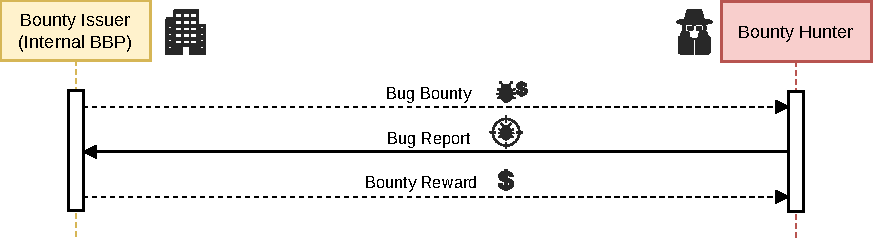
\includegraphics[scale=0.65]{bbp/bbp-internal-icons-small}
%\caption[Interazione nel caso di \internalBBP]{interazione tra \BI e \BH nel caso di \internalBBP e \bugreport valido.}
%\label{figure:bbp-internal}
%\end{figure}
%
%\begin{figure}[tbhp]
%\centering
%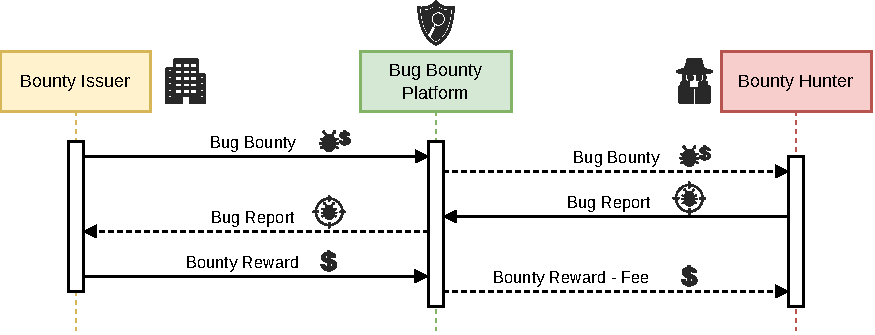
\includegraphics[scale=0.65]{bbp/bbp-platform-icons-small}
%\caption[Interazione nel caso di \bugbountyplatform]{interazione tra \BI e \BH nel caso di \bugbountyplatform e \bugreport valido.}
%\label{figure:bbp-platform}
%\end{figure}

\begin{figure}[tbhp]%
\centering
\subfloat[Interazione diretta tramite \emph{internal \acs{BBP}}.]{%
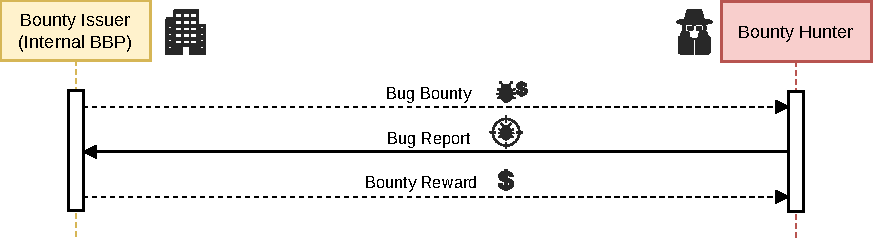
\includegraphics[scale=0.80]{bbp/bbp-internal-icons-small}%
\label{figure:bbp-internal}%
}\\
\subfloat[Interazione indiretta tramite \emph{bug bounty platform}.]{%
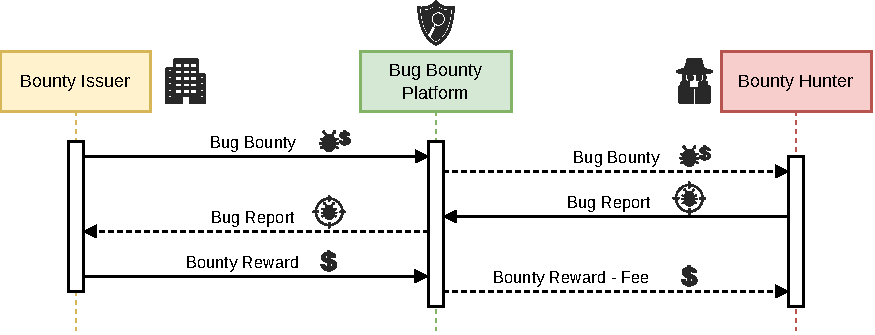
\includegraphics[scale=0.80]{bbp/bbp-platform-icons-small}%
\label{figure:bbp-platform}%
}%
\caption[Interazione tra \emph{\acs{BI}} e \emph{\acs{BH}}]{interazione tra \BI e \BH nel caso di \bugreport valido.}
\label{figure:bbp-interaction}
\end{figure}

Possiamo classificare i \BBP in base al fatto che l'interazione tra il \BI e il \BH avvenga direttamente o tramite da un intermediario:

\begin{itemize}

\item \InternalBBP: sono \BBP gestiti direttamente dal \BI \cite{hoffman2021bountychain}; in tal caso, come possiamo osservare in \cref{figure:bbp-internal}, la comunicazione tra il \BI e il \BH avviene in modo diretto.
%solo le aziende di grandi dimensioni - come Google, Meta o Microsoft - possono permettersi di gestire dei programmi interni \cite{walshe2023bountythesis3}.

\item \BugBountyPlatform: sono piattaforme che fungono da mediatore tra il \BI ed il \BH \cite{hoffman2021bountychain}; di conseguenza, come illustrato in \cref{figure:bbp-platform}, la comunicazione avviene in modo indiretto.
Esempi di queste piattaforme sono \HackerOne, \Intigriti, \Bugcrowd, \Synack e \Yogosha \cite{walshe2023bountythesis3, walshe2020bountypaper}. 
%aziende di piccole o media dimensioni di solito si affidano a questo genere di soluzioni \cite{walshe2023bountythesis3, walshe2020bountypaper};

\end{itemize}

\subsection{Adozione}

Alla fine del 1995, l'azienda statunitense Netscape fu la prima a implementare un \BBP al fine di individuare eventuali difetti software presenti nel web browser Netscape Navigator; tuttavia, bisognerà attendere i primi anni duemila affinché l'uso di questi programmi cominci a diffondersi maggiormente \cite{hoffman2021bountychain}.
Ad oggi, le aziende di piccole o medie dimensioni che desiderano avviare un \BBP si affidano a una delle varie \bugbountyplatform esistenti, mentre solo le aziende di grandi dimensioni -- come \GoogleBBP, \MetaBBP o {\MicrosoftBBP} -- possono permettersi di gestire dei programmi interni \cite{walshe2023bountythesis3}.

%\subsection{Vantaggi e limitazioni}

\subsection{Vantaggi}

L'adozione dei \BBP offre alla comunità degli \hacker una via legale per la segnalazione delle \vulnerability, disincentivando così l'utilizzo del mercato nero \cite{fryer2017bugbounty, walshe2020bountypaper, walshe2023bountythesis3} e amplificando la probabilità che vengano scoperti \bug che altrimenti sarebbero rimasti nascosti agli occhi degli eventuali team di cybersecurity a disposizione delle aziende \cite{walshe2020bountypaper}.

\subsection{Limitazioni}

\medskip

Una delle limitazioni più importanti degli \internalBBP è il fatto che, una volta che il \BI ha ricevuto il \bugreport, questi è fortemente incentivano a considerare i bug segnalati come poco critici o non validi al fine di ridurre al minimo la ricompensa per il \BH \cite{canidio2021verioss, akgul2023bughunters}; questa situazione rende il mercato inefficiente per i \BH che risultano, di conseguenza, portati a cercare altre vie per la vendita dei bug \cite{canidio2021verioss}.

\medskip

Una risposta a questo problema arriva dalle \bugbountyplatform che, in quanto mediatori imparziali, dovrebbero riuscire ad ottenere ricompense più adeguate per i \BH \cite{canidio2021verioss, akgul2023bughunters}. 

\medskip

Tuttavia anche le piattaforme bug bounty presentano delle criticità \cite{badash2021blockbounty}:
\begin{enumerate}

\item Costi aggiuntivi: la maggior parte di queste piattaforme tassa in modo non trascurabile le ricompense elargite ai \BH.

\item Poca trasparenza: le piattaforme spesso non delineano chiaramente il meccanismo di valutazione delle \vulnerability segnalate; questa mancanza di trasparenza può risultare in un trattamento preferenziale verso i \BI, che sono loro clienti.

\item Rischi di sicurezza: l'introduzione di un intermediario nell'interazione tra \BI e il \BH aumenta il rischio di divulgazione non autorizzata di informazioni sensibili.

\end{enumerate}

\subsection{Divulgazione delle vulnerabilità}

I \BBP possono anche essere distinti in base all'approccio adottato per la divulgazione della \vulnerability identificate dai \BH; in particolare, esistono tre principali approcci di divulgazione \cite{lisi2022ard, cavusoglu2007vulndisc}:
\begin{itemize}

\item \FullVendorDisclosure: la \vulnerability viene comunicata esclusivamente al \BI.

\item \FullPublicDisclosure: la \vulnerability viene resa pubblica immediatamente dopo la sua identificazione, senza concedere al \BI alcun tempo per la correzione.

\item \ResponsibleDisclosure: la \vulnerability è inizialmente comunicata esclusivamente a una terza parte fidata, incaricata di verificarne la validità; se questa viene confermata, il \bugreport viene inoltrato al \BI, al quale viene dato un periodo di tempo prestabilito per correggere il problema nel proprio sistema software prima della divulgazione pubblica.
\end{itemize}

L'utilizzo dell'approccio \fullvendordisclosure non stimola adeguatamente il \BI a rimuovere tempestivamente le \vulnerability individuate: un \BI negligente potrebbe posticipare per un lungo periodo la correzione del software, lasciando in tal modo i propri utenti esposti al rischio di attacchi \cite{lisi2022ard, cavusoglu2007vulndisc}.

\medskip

Seguendo il \fullpublicdisclosure, il \BI è motivato a realizzare un aggiornamento correttivo il prima possibile, onde evitare una compromissione della propria reputazione \cite{cavusoglu2007vulndisc, arora2010vulndisc}; tuttavia, diventa concreto il rischio che potenziali attaccanti sfruttino la \vulnerability, ormai di dominio pubblico, prima che il \BI riesca ad agire \cite{lisi2022ard, cavusoglu2007vulndisc, arora2010vulndisc}.

\medskip

L'impiego del \responsibledisclosure incentiva il \BI attraverso il potenziale danno di immagine dovuto alla diffusione pubblica della \vulnerability, fornendogli al contempo il modo di correggerla prima che attori malevoli possano sfruttarla. Quest'approccio, purtroppo, non risulta privo di problemi: il suo utilizzo presuppone il coinvolgimento di un mediatore tra \BI e \BH, presentando così limitazioni paragonabili a quelle associate all'utilizzo delle \bugbountyplatform.

\subsection{Riferimenti bibliografici aggiuntivi}

Per eventuali approfondimenti sui \BBP, oltre ai lavori già citati nel testo, si rimanda ai seguenti documenti: 
\begin{itemize}

\item Walshe (2023), "Supporting Data-driven Software Development Life-cycles with Bug Bounty Programmes" \cite{walshe2023bountythesis};

\item Malladi \etAl (2020), "Bug Bounty Programs for Cybersecurity: Practices, Issues, and Recommendations" \cite{malladi2020bugbounty}.

%\item Fryer e Simperl (2017), "Web Science Challenges in Researching Bug Bounties" \cite{fryer2017bugbounty}.

\end{itemize}

\section{Protocollli di fair exchange}

%----------SUGGERIMENTI-SUL-CONTENUTO----------%
%Iniziamo con l'introduzione di concetti, definizioni e teorie fondamentali che costituiscono le basi del nostro lavoro. Questa sezione potrebbe includere, ad esempio, modelli matematici e teoremi essenziali per la comprensione della tesi.
%
%\medskip
%
%È importante tenere a mente che non stiamo scrivendo un libro di testo: ogni volta che introduciamo un termine o un concetto sarà sufficiente fornirne una breve spiegazione e includere un riferimento bibliografico; in tal modo il lettore potrà approfondire autonomamente l'argomento \cite{tuni2019guide}.
%----------------------------------------------%

\section{Blockchain}

%----------SUGGERIMENTI-SUL-CONTENUTO----------%
%Iniziamo con l'introduzione di concetti, definizioni e teorie fondamentali che costituiscono le basi del nostro lavoro. Questa sezione potrebbe includere, ad esempio, modelli matematici e teoremi essenziali per la comprensione della tesi.
%
%\medskip
%
%È importante tenere a mente che non stiamo scrivendo un libro di testo: ogni volta che introduciamo un termine o un concetto sarà sufficiente fornirne una breve spiegazione e includere un riferimento bibliografico; in tal modo il lettore potrà approfondire autonomamente l'argomento \cite{tuni2019guide}.
%----------------------------------------------%

% DLT

% Blockchain

% Smart Contracts

\section{Lavori precedenti}

%VeriOSS paper 1

%VeriOSS paper 2

%FOSS

%BBP e FOSS

%Problema del nostro approccio: è full public disclosure.

%----------SUGGERIMENTI-SUL-CONTENUTO----------%
%Successivamente, se la tesi è una diretta continuazione di articoli o progetti di ricerca preesistenti, esporremo questi lavori evidenziando come la nostra ricerca si sviluppi a partire dalle loro fondamenta.
%----------------------------------------------%

\section{Metodi e tecniche utilizzate}

%----------SUGGERIMENTI-SUL-CONTENUTO----------%
%In questa sezione descriveremo i metodi e le tecniche adottate nel corso della tesi, quali le analisi statistiche o i metodi di sviluppo software utilizzati per portare avanti il nostro progetto.
%
%\medskip
%
%Nel caso di un progetto implementativo, descriveremo la metodologia di sviluppo impiegata (es. Agile, Waterfall, TDD, BDD) e come questa abbia influenzato il processo di implementazione.
%----------------------------------------------%

% Verifica formale

\section{Tecnologie utilizzate}

%----------SUGGERIMENTI-SUL-CONTENUTO----------%
%Concludiamo il capitolo presentando le tecnologie, inclusi gli strumenti software e hardware, impiegati nella nostra ricerca, spiegando il loro ruolo e come hanno contribuito al raggiungimento degli obiettivi della tesi.
%
%\medskip
%
%Nel caso di un progetto implementativo, in questa sezione elencheremo i linguaggi di programmazione, i framework, i database e altri strumenti utilizzati per lo sviluppo e il test del software. Ogni scelta andrà motivata illustrando quali sono i vantaggi per il nostro progetto.
%----------------------------------------------%

% Ethereum

% Solidity

% Solidity SMTChecker

% Chainlink

% IPFS

% Remix

\section{Riassunto del capitolo e conclusioni}

%----------SUGGERIMENTI-SUL-CONTENUTO----------%
%Alla fine di ogni capitolo includeremo un breve riassunto del suo contenuto, una riflessione su come quanto trattato contribuisca agli obiettivi generali della tesi e, per concludere, un'anticipazione di come i capitoli successivi faranno uso di quanto introdotto in quello corrente (in tal modo metteremo in evidenza come questi sono tra loro collegati) \cite{zobel2015writing}.
%----------------------------------------------%